\section{Logistics}
\label{sec:fdsp-tc-log}


% orig 2nd draft Transporting equipment and people underground is one of the more challenging aspects of the \dword{lbnf}/\dword{dune} endeavor. Access underground goes through the mile long Ross shaft, which is now undergoing renovation. The shaft is outfitted with a single cage for people and materials and two skips that are needed to remove the rock underground. Planning for using the cage is important to making \dword{lbnf}/\dword{dune} a success. Given the enormous cost of the \dword{cf} contracts and the large cost of any inefficiencies in construction, the overall coordinator of the Ross Shaft for \dword{lbnf}/\dword{dune} will be the \dword{cf} \dword{cmgc}. Both \dword{lbnf} and \dword{dune} will also have a large number of contractors, institutions, and scientists who will need to bring equipment and materials underground. \dword{lbnf}/\dword{dune} will establish a logistics organization in South Dakota near \dword{surf} to facilitate the flow of material and people to the underground area. This organization will be responsible for receiving all goods for \dword{lbnf} (except CF) and \dword{dune},for coordinating the transport of this material underground with the \dword{cf}-\dword{cmgc}, and for coordinating personnel usage of the Ross cage with the \dword{cf}-\dword{cmgc}. 

Transporting equipment and people underground is one of the more challenging aspects of the \dword{lbnf} and \dword{dune} endeavor. The mile-deep Ross Shaft, currently undergoing renovation, provides access underground. The shaft is outfitted with a hoist that controls a single cage for transporting people and materials and two skips that are used to remove the underground rock. The cage is new.  Given the enormous cost of the \dword{cf} contracts and the large cost of any inefficiencies in construction, scheduling use of the shaft is important to making \dword{lbnf} and \dword{dune} successful. The  \dword{lbnf} \dword{cf} \dword{cmgc} will be the overall coordinator of the Ross Shaft for \dword{lbnf} and \dword{dune}. In addition to  \dword{cmgc} personnel,  many \dword{lbnf} and \dword{dune} contractors and institutions  will need to bring personnel, equipment and materials underground. \dword{lbnf} and \dword{dune} will establish a logistics organization and a warehouse  
\fixme{a facility or an organization? \dword{sdwf}? I added warehouse. anne} 
in South Dakota near \dword{surf} to facilitate the flow of people and material to the underground area. This organization will be responsible for (1) receiving all goods for \dword{lbnf} (except \dword{cf}) and \dword{dune}, (2) coordinating the transport of this material underground with the \dword{cf}-\dword{cmgc}, and (3) coordinating use of the Ross shaft with the \dword{cf} \dword{cmgc}. 

\fixme{schematic map of wdwf, Ross headframe, any other locations, would be helpful}

%\begin{dunetable}
%[Logistics Specifications]
%{ll}
%{tab:table-Log-Req}
%{Table of logistics specifications.}
%Specifications &  \\ \toprowrule
%Material Handling & Comply with the SURF Material %Handling Specification \\ \colhline
%CMGS coordination & Provide CMGC with two-week notice %of shipments to SURF \\ \colhline
%Stage DUNE Shipments & Provide a one-month local %buffer of DUNE materials \\
%\colhline
%\dword{apa} Storage & Provide storage space for 150 %\dword{apa}s in a clean environment \\
%\colhline
%Inventory & Provide an inventory system accessible to %the collaboration \\
%\end{dunetable}
 %\fixme{Specifications table needs to be converted to official format}
 
Figure~\ref{fig:logistics-material-flow} shows a high-level overview of the material flow to the Ross headframe. Freight is delivered to a central warehouse, the \dword{sdwf}, except for possibly the cryogenic equipment. 
 The materials are then transported in a just-in-time fashion to the Ross headframe where they are brought underground. 
 %For the detector, the \dword{apa}, electronics and \dword{pd} components %will %also be are shipped to the \dword{itf} where they are assembled and then shipped %back  to \dword{sdwf}.
 
\begin{dunefigure}[Material flow diagram for logistics ]{fig:logistics-material-flow}
  {Material flow diagram for the \dword{lbnf} and \dword{dune} logistics.}
 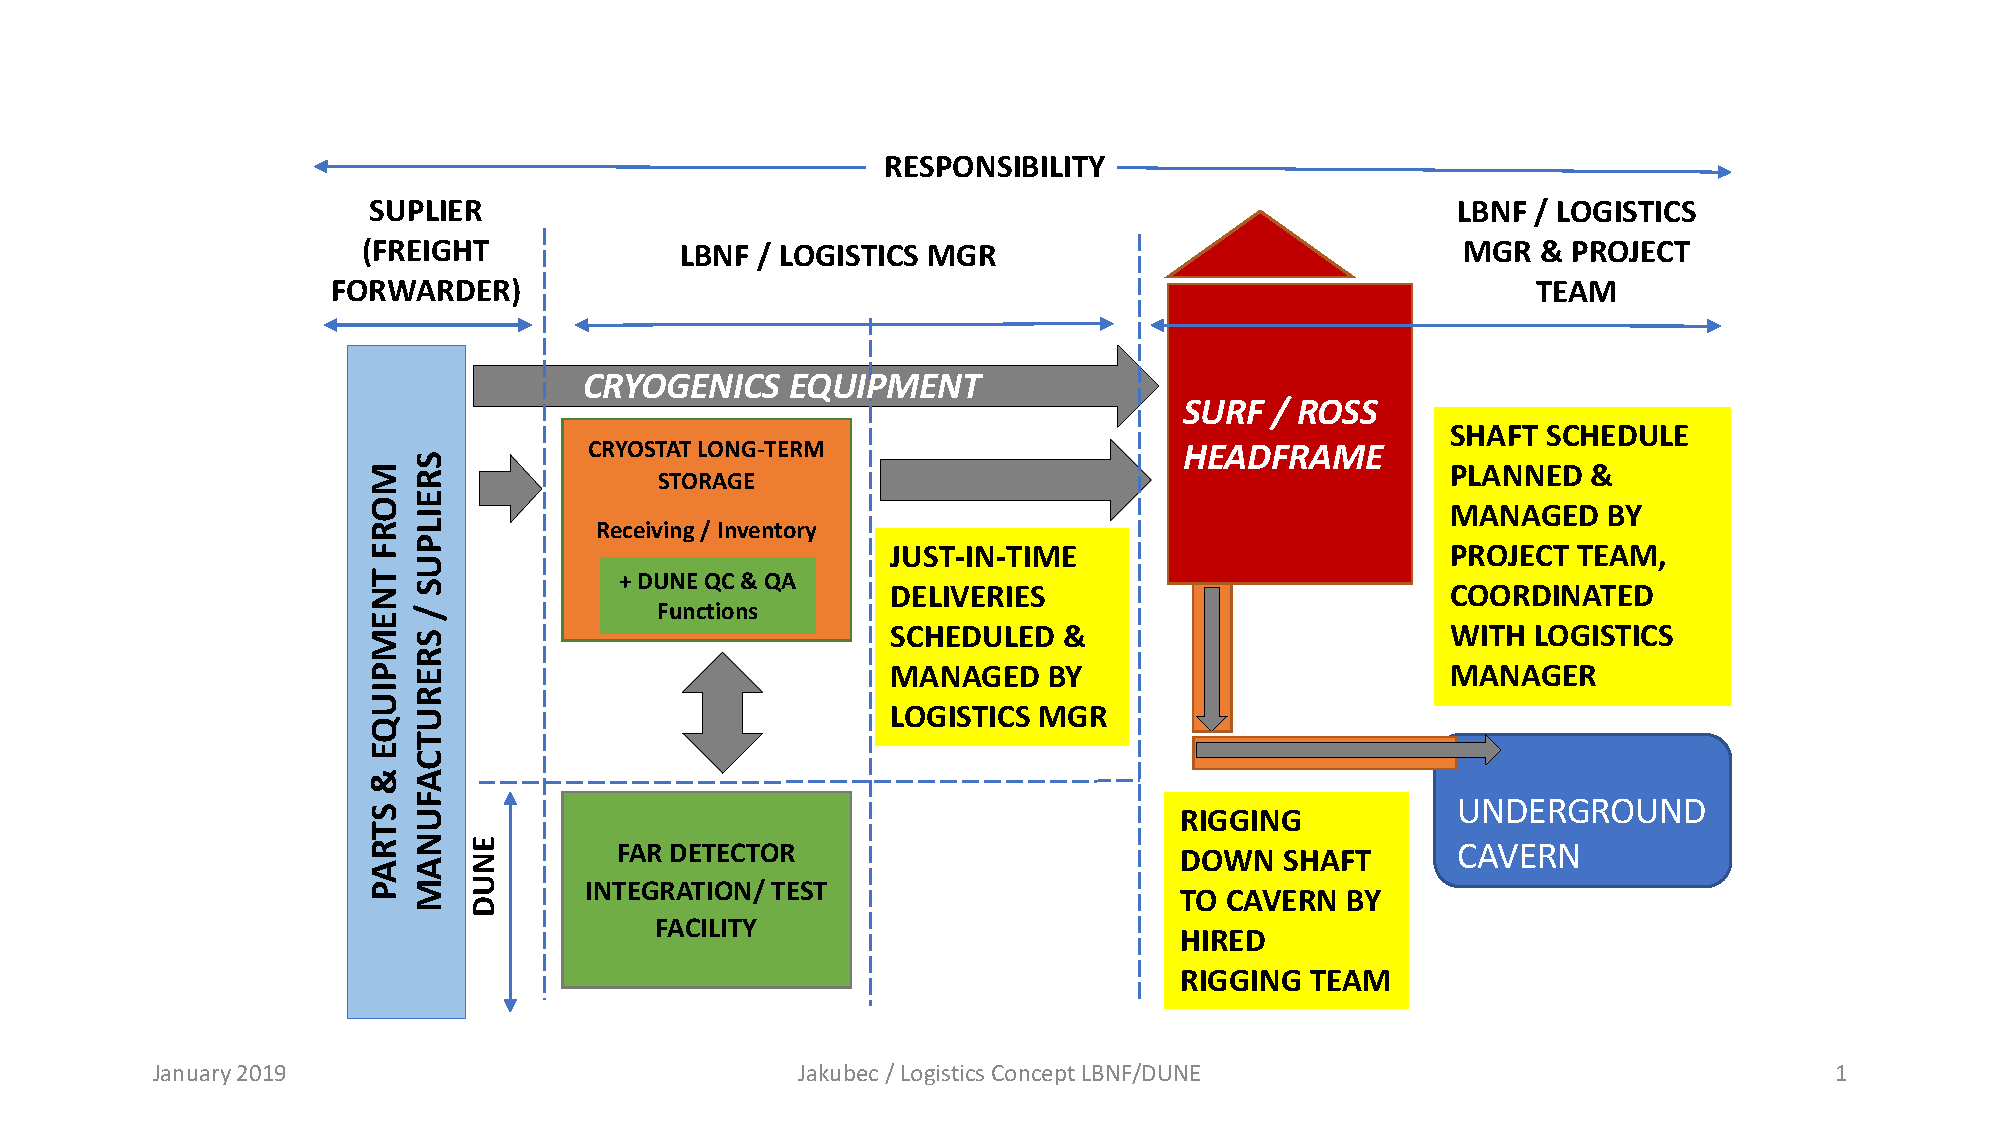
\includegraphics[width=\textwidth]{logistics-material-flow}
\end{dunefigure}

\fixme{how close does SDWF have to be to surf?   Is the orange the SDWF? Should use same name everywhere. anne.}

%%%%%%%%%%%%%%%%%%%%%%%%%%%%  
\subsection{Logistics Planning}
\label{sec:fdsp-tc-logPln}

\dword{lbnf} and \dword{dune} logistics oversees transportation of the cryostat (steel, foam, and membrane), the cryogenics system, the detector, and all related infrastructure not provided by %facilities. 
the \dword{cf}. \dword{lbnf} specifically oversees the cryostat and cryogenics system, which %will not be 
are  discussed in detail in %this 
the \dword{lbnf} \dword{tdr}; 
\fixme{add ref} because \dword{lbnf} material dominates the logistics, we present a summary. % is required. 
The %cryostat 
steel structure for each cryostat requires %bringing 
roughly 1,800 individual steel pieces, % underground, 
some which weigh up to \SI{7.5}{t}, as well as \SI{125}{t} of bolts to assemble the steel pieces. The internal structure, which includes the foam insulation and the thin stainless steel membrane, %will 
requires transporting roughly 4,000 boxes, 
\fixme{per cryostat?} each roughly 1.5 $\times$ 3.5 $\times$ 1.2 m$^3$. The plan for cryostat installation, at present, calls for all components to be warehoused  in South Dakota \fixme{SDWF? be more specific} before installation begins. %This means that t
The logistics operation will  therefore need roughly $\SI{5,000}{m^2}$ of warehouse space approximately two years before installation of the first DUNE \dword{detmodule} begins. By the time DUNE detector components start arriving, most of the cryostat boxes will have been removed from the warehouse, leaving ample space for the detector and cryogenics components. Additional space may be required if the boxes for the second cryostat arrive before  \dword{detmodule} \#1 installation is complete; several buildings of the required size are available in the area around \dword{surf}. % if expansion is required.


\begin{dunefigure}[Simplified model of the Ross Cage]{fig:fdsp-tc-Cage}
  {Simplified Ross Cage model.}
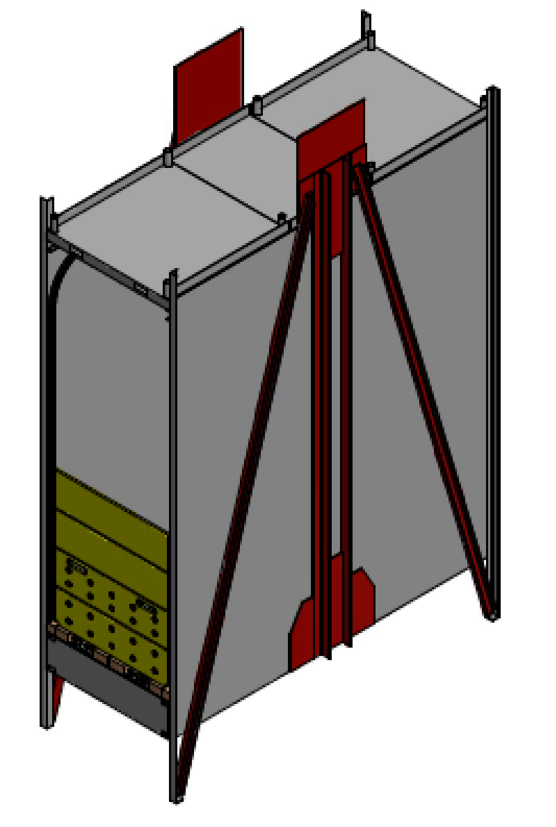
\includegraphics[width=.5\textwidth]{Cage-view}
\end{dunefigure}
%
\begin{dunetable}
[Ross Cage specifications]
{cc}
{tab:table-Ross-Cage}
{Ross Cage parameters.}
Ross Cage Parameters &  
\\ \toprowrule
Inside height &  3.6 m\\ \colhline
Inside depth & 3.7 m \\ \colhline
Inside width & 1.38 m \\
\colhline
Weight limit&  5,897 kg \\
\colhline
Round trip time & 17 min\\ \colhline
\end{dunetable}
\fixme{put table and image together - David D? Figure needs dimensions one way or another}

%All material brought underground must conform to the \dword{surf} Facility Access Specification \cite{bib:docdb328}. This document defines the limitations on dimensions and weights for all materials to be transported underground.  The most important limitations, which are described in detail in the specification document, relate to the Ross shaft and Ross cage. It is possible to bring material down the shaft underneath the cage as a slung load, but this is a much slower process and requires careful planning, detailed procedures, and review. The \dword{dune} \dword{apa}, for example, requires this special handling because they are too tall to fit in the cage. Most material should be brought underground inside the cage. Figure \ref{fig:fdsp-tc-Cage} shows an image of the new Ross cage and Table \ref{tab:table-Ross-Cage} summarizes its parameters. The round trip travel time for the Ross cage is 17 minutes and this is dominated by loading and unloading time. The time needed to load, lower, and unload any slung load is more than an hour round trip as each step is much longer. 
The \dword{surf} Facility Access Specification~\cite{bib:docdb328} defines the limitations on dimensions and weights for all materials to be transported underground, the most stringent of which are set by the Ross shaft and cage. It is possible to bring material down the shaft underneath the cage as a slung load, but this is a much slower process and requires careful planning, detailed procedures, and review. The \dword{dune} \dword{apa}s, for example, require this special handling because they are too tall to fit in the cage. Most material will be brought underground inside the cage. Figure \ref{fig:fdsp-tc-Cage} illustrates the new Ross cage and Table \ref{tab:table-Ross-Cage} summarizes its parameters. \fixme{fix if fig and tab get merged} The round trip travel time for the Ross cage is 17 minutes, which is dominated by loading and unloading time. \fixme{what are actual travel times up and down? Load/unload times must vary depending on what the load is.} Slung loads will require more than an hour round trip .

\fixme{sorry, I did not keep the orig pgraph here}

The Ross headframe has no loading dock, so careful coordination is required. All materials transported to it must arrive on a flatbed or curtain-sided chassis, where a forklift can unload  the items. The logistics team coordinates all deliveries to the headframe, and the \dword{cf}-\dword{cmgc} coordinates all transport from there down the shaft.  Most material will be delivered first to the \dword{sdwf}, where a central inventory system will capture data about the shipments.  All deliveries, either from this warehouse or direct to the Ross headframe, require (1) coordination with the logistics team, and (2) minimum two weeks prior notice, per an advance delivery plan \fixme{ref}.  The logistics team will provide a shipping manual \fixme{ref} to \dword{dune} institutions. The institutions must provide shipping data and consign cargo according to the guidelines so that the logistics team can monitor progress. 



In \dword{protodune}-\dword{sp}, delays in shipping and customs resulted in up to three weeks delay in the arrival of some parts, which necessitated significant re-planning of the installation work. To prevent this from becoming a much larger problem in \dword{dune}, we plan a minimum one month buffer of materials. This buffer will allow advance planning for the underground work, %can be planned well in advance, knowing 
with confidence that all materials will be available as needed. %This will require that sufficient space be available in the warehouse and underground at \dword{surf} to house the material buffer. Many small parcels will arrive at the warehouse from different sources. 
Sufficient space must be made available in the warehouse and in the underground area  to house this material. % buffer. Many small parcels will arrive at the warehouse from different sources.
The warehouse staff will de-consolidate or consolidate arriving cargo into larger boxes and crates, as needed, for  delivery to %the \dword{itf} or 
\dword{surf}, following established % \dword{itf} or \dword{surf} 
delivery plans, to make the most efficient use of available trucks and the Ross Shaft. %hoist. 
\fixme{do we want to refer to the hoist, the cage or the shaft?}


\begin{dunefigure}[Underground space needs during installation setup]{fig:fdsp-tc-setup}
  {Image showing the cavern on end opposite of the detector during the installation setup phase.  Half the space will be used for the cryostat work and half for storage of the detector infrastructure. The material outside the cavern must be stored in the logistics warehouse.}
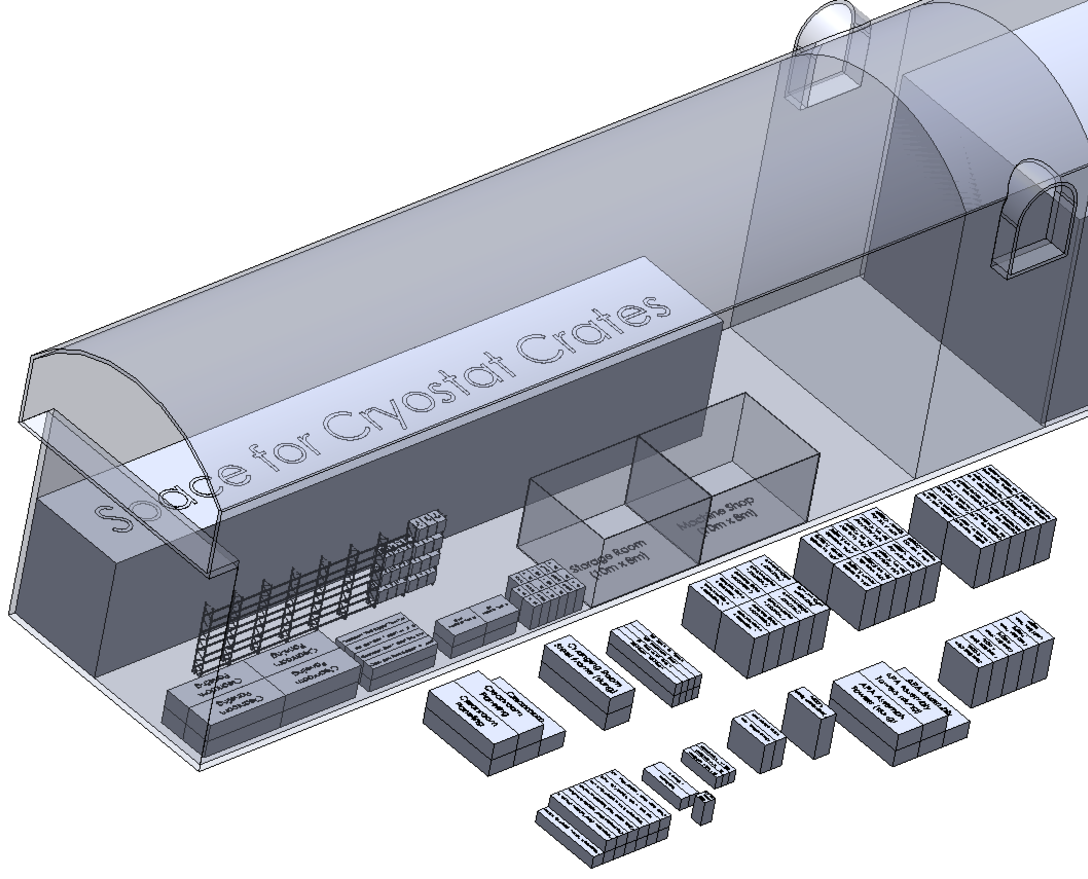
\includegraphics[width=.9\textwidth]{Material-Setup}
\end{dunefigure}
%
\fixme{in fig caption:  the cavern on end opposite of the detector - ?? And is logistics warehouse the sdwf? Also, almost all text in fig is unreadable.}

To discover how much space is needed for storage and how much hoist time must be dedicated to \dword{dune}, a detailed inventory of all detector equipment and \dword{dune} infrastructure is needed. The list of %all the 
materials has been solicited from all consortia and technical coordination. The entries in the inventory spreadsheet are organized as ``loads'' for the Ross shaft where a load is a crate or set of boxes that will be transported underground in one trip, either in the %hoist
cage or as a slung load~\cite{bib:docdb8426}. 
Information captured in the load spreadsheet includes the number of %hoist 
trips, type of trip (slung load or cage), package dimensions, weight and type of package (crate, pallet, box, or carton). 

The load list at present predicts 1,600 hoist trips and approximately two  months of cage time, most of which is spread over one year. Installation %operation 
(see Figure \ref{fig:high-level-schedule}) for the \dword{spmod} %detector 
will span two years, so we divide the logistics planning into three  %several 
phases: % is prudent.  The load information is divided into 
(1) the \dword{cuc} setup phase, (2) the installation setup phase, and (3) the detector installation phase. For each phase, a model was generated to show how much material can be stored underground outside the work area and how much material must be stored on the surface. These models set the space requirements for the logistics on the surface. The phase with the largest amount of material to transport is the detector setup phase. \fixme{not defined, detector installation?}  Figure \ref{fig:fdsp-tc-setup} shows the model of the underground area and the required boxes for surface storage for the first third of the setup. This represents the first month of installation setup and shows that roughly 1,000 m$^2$\ of warehouse space will be needed for \dword{dune} at this time.  The %warehouse 
\dword{sdwf} will also need space to store up to 150 \dwords{apa}, %in addition to the space needed to receive and ship equipment underground. This 
adding %an additional 
700 m$^2$ to the 1,000 m$^2$. %\ to needed warehouse area. 


%%%%%%%%%%%%%%%%%%%%%%%%%%%%
%\subsection{Logistics Quality Assurance and Quality Control}
\subsection{Logistics Quality Control}
\label{sec:fdsp-tc-log-qaqc}


%\dword{protodune} was an extremely useful exercise in general, but we can draw only a few conclusions about \dword{dune} logistics %because 
%since shipping to Europe differs from shipping to South Dakota and different staff will be responsible for receiving and transport. %the CERN receiving and transport divisions will not be used for \dword{dune}. 
The \dword{protodune} experience offers a couple of significant lessons regarding logistics.

%The full list of %lessons learned is found in the 
%ProtoDUNE-SP lessons learned is in~\cite{bib:docdb8255}. %spreadsheets. 
%The most important lessons learned from \dword{protodune} logistics are: % listed below.
\begin{enumerate}
%\item Lack of a central inventory system made it impossible to track shipments.
%\item Delays in shipping meant that the installation work could not be planned and parts were installed as they arrived. 
\item A central inventory system is essential for tracking  shipments.
\item It is important to avoid delays in shipping because installation work cannot proceed as planned. 
\end{enumerate}

%To address these issues, a central inventory system will be implemented at the logistics warehouse facility, and a minimum one month material buffer will be required from the consortia in South Dakota.
The central inventory system  implemented at the \dword{sdwf}  and the minimum one month material buffer are the plans we have in place to prevent repetition of the problems we experienced with \dword{pdsp}.   The full list of lessons learned from \dword{pdsp} is in~\cite{bib:docdb8255}. 

We do not foresee any component testing at the \dword{sdwf}, %in the warehouse, 
so the scope of the \dword{qc} work there is limited to two functions. %A \dword{qa}/\dword{qc} component, however, will be required at receiving. 
%However, a critical \dword{qc} check there %at the logistics facility 
%will 
The facility will ensure that all materials to be shipped to the Ross headframe will fit in the cage, or %. Moreover, 
if a slung load is needed, %the facility will confirm 
that the necessary procedures are in place and approved before any material is transported. % to \dword{surf}. 
It will also %The other primary \dword{qc} function performed at the logistics facility is to 
inventory all received shipments. % described below.

%The contribution in kind model of this project makes logistics and inventory control as well as gathering of the relevant construction data extremely complex. Therefore, the logistics (inventory) control and collection of scientific data  must be controlled by independent systems. 
%The logistics supply chain will be controlled by the contributors' freight forwarding system until supplies arrive at the \dword{sdwf}, which has yet to be defined/established.  \dword{sdwf} will be the ultimate point of capture for all \dword{lbnf}/\dword{dune} parts/equipment except possibly for the cryogenic system, given the contractual requirements. The inventory process at the \dword{sdwf}, the \dword{itf} and the \dword{surf} receiving at Ross Shaft will be controlled by one \dword{wms}. 

The contribution-in-kind model of this project complicates logistics and inventory control and the gathering of the relevant construction data. Therefore, the inventory control and the collection of scientific data 
\fixme{scientific data? is this testing data?} must be controlled by independent systems. 
Until materials arrive at the \dword{sdwf} or \dword{surf} (if directly shipped), the contributors' freight forwarding system will control the logistics supply chain, which has yet to be defined.  \dword{sdwf} will be the ultimate point of capture for all the materials except possibly for the cryogenics system, given its special contractual requirements. A central \dword{wms} will control the inventory process at the \dword{sdwf} and the \dword{surf} receiving at the Ross headframe. 

%The \dword{wms} will provide basic receiving, inventory control, and shipping status for all parts and equipment delivered to \dword{sdwf}. That will include pre-assembled equipment, which will enter as new parts from \dword{itf} as created by the integration work. The \dword{qc}/\dword{qa}, manufacturing, and other relevant data required by the \dword{dune} collaborators will be stored in a separate, as yet undefined and undeveloped, \dword{dcdb}.  The \dword{dcdb} is independent of the \dword{wms} system, and the relevant contributing consortia are responsible for transferring the required data before shipment from supplier to the \dword{dcdb}.  The \dword{wms} database will provide the relevant logistics data to the \dword{dcdb}. The form of data transfer is not yet determined. All \dword{qc}/\dword{qa}, test, and other relevant manufacturing data will be directly input into \dword{dcdb} and will be the responsibility of the different contributing consortia. \dword{dune} must provide a \dword{qc}/\dword{qa} process for all parts/equipment received at the warehouse after being inventoried. That \dword{qc}/\dword{qa} data must be transferred directly to \dword{dcdb} by \dword{dune}.  The \dword{dcdb} will be an integral part of the logistics, assembly, and \dword{qc}/\dword{qa} system. It must provide the \dword{itf} shipping (supply) and assembly reports and create the new equipment denomination for the \dword{wms} to register.  The \dword{dcdb} will document the \dword{itf} sub-assembly process in its entirety.
The \dword{wms} will control basic receiving, inventory control, and shipping status for all components, parts, and equipment delivered to the \dword{sdwf}, %including equipment  pre-assembled at the \dword{itf}, 
which will be entered \fixme{Enter first as components upon receipt, then re-enter as assembly when ready to ship? Fix now that there's no ITF} as new parts created by the integration work. The \dword{qc}, %/\dword{qa}, 
\fixme{I don't think you want QA  here} manufacturing, and other %relevant 
data required by the \dword{dune} collaborators will be stored in a separate, as yet undefined  %and undeveloped, 
\dword{dcdb}, independent of the \dword{wms} system. 

The consortia are responsible for transferring the required data from the supplier to the \dword{dcdb} prior to shipment.  The \dword{wms} database will provide the associated logistics data to the \dword{dcdb} (the form of data transfer is not yet determined). 
\fixme{wms and dcdb are independent or not? I'm confused. Anne}
All \dword{qc}, %dword{qa}, 
test, and other relevant manufacturing data will be directly input into \dword{dcdb} and will be the responsibility of the different contributing consortia.  
\fixme{wait, isn't this info in a different system? Finish pgraph after resolved}
\dword{dune} must provide a \dword{qc}/\dword{qa} process for all parts and equipment received at the warehouse after being inventoried. That \dword{qc}/\dword{qa} data must be transferred directly to \dword{dcdb} by \dword{dune}.  The \dword{dcdb} will be an integral part of the logistics, assembly, and \dword{qc}/\dword{qa} system. It must provide the \dword{itf} shipping (supply) and assembly reports and create the new equipment denomination for the \dword{wms} to register.  The \dword{dcdb} will document the \dword{itf} sub-assembly process in its entirety. \fixme{fix now that there's no ITF}

The new sub-assembled items will be inventoried in \dword{wms} as new items during the warehouse receiving process. 
The \dword{jpo} installation management team will be responsible for providing a shipping (supply) report to the warehouse for scheduling of parts/equipment shipments to \dword{surf}.
The shipments from \dword{sdwf} to \dword{surf} will be inventoried as received at \dword{surf} in \dword{wms}. 
The \dword{dune} installation team must transfer the relevant \dword{qc}, %/\dword{qa}, 
test, and installation status data to the \dword{dcdb} directly.
To capture all relevant construction and logistics data on parts and equipment, logistics information should follow this process:

\begin{itemize}
\item The consortia %must 
enter data related to %any 
shipments to the \dword{sdwf} into the \dword{wms}.
\item The logistics team at \dword{surf} inventories the shipments from \dword{sdwf} % to  \dword{surf} will be inventoried as received at \dword{surf} 
in the \dword{wms}.
\item The \dword{jpo} installation management team %will be responsible for 
provides a shipping (supply) report to the %warehouse 
\dword{sdwf} for scheduling shipments %of parts/equipment 
to \dword{surf} two weeks in advance of any shipment.
\end{itemize}
\fixme{2nd item: who at surf inventories this? I guess: logistics team? 3rd item: clarify what shipping report contains -- how is it used to schedule shipments?}

\fixme{a flow diagram of the QA/QC process data, QA/QC manufacturer tests, install status, WMS, new eqp denomination, reports on ship/supply/assy, DCDB, etc. would be helpful.}

%%%%%%%%%%%%%%%%%%%%%%%%%%%%
\subsection{Logistics Safety}
\label{sec:fdsp-tc-log-safety}

%The \dword{lbnf}/\dword{dune} logistics facility is operated by \dword{sdsd}  as a Fermilab facility, but because of the international connections, we also follow CERN HSE, Fermilab ES\&H, and \dword{surf} ES\&H regulations.  Work is in progress to combine the three into a coherent list of codes and requirements. The \dword{dune} Project ES\&H Coordinator has overall ES\&H oversight responsibility for the \dword{dune} Project.  This person coordinates any activities and facilitates the resolution of any issues that cut across various divisions and institutions and subject to the requirements of the \dword{doe} Workers Safety and Health Program, Title 10, Code Federal Regulations (CRF) Part 851 (10 CFR 851). These requirements are promulgated through the Fermilab Directors Policy Manual and Fermilab ES\&H manual (FESHM), which align with the \dword{surf} ES\&H Manual.  Using the NOvA Far Detector Laboratory as a guideline for remote facilities, several other key documents guide the Logistics Center Safety Program.  The Building Safety Plan combines all building specific documents in a single folder:
The \dword{lbnf}/\dword{dune} logistics facility
\fixme{the warehouse?}  is operated by \dword{sdsd}  as a Fermilab facility, but because of the international collaboration, we  follow \dword{esh} regulations from CERN and \dword{surf} in addition to Fermilab's.  Work is in progress to combine the three into a coherent list of codes and requirements. The \dword{dune} Project \dword{esh} Coordinator has overall \dword{esh} oversight responsibility for the \dword{dune} Project.  This person coordinates any \dword{esh} activities and facilitates the resolution of any issues that are subject to the requirements of the \dword{doe} Workers Safety and Health Program, Title 10, Code Federal Regulations (CRF) Part 851 (10 CFR 851), and that cut across various divisions \fixme{divisions of what?} and institutions. These requirements are promulgated through the Fermilab Director's Policy Manual \fixme{ref} and Fermilab \dword{esh} manual (FESHM) \fixme{ref}, which aligns with the \dword{surf} \dword{esh} manual.  Using the \dword{nova} Far Detector Laboratory as a guideline for remote facilities, several other key documents guide the Logistics Center Safety Program.  The Building Safety Plan \fixme{ref} combines all building specific documents in a single folder:

\begin{enumerate}
\item	Fire Safety and Building Emergency Evacuation Plan, which includes the fire evacuation plan, fire safety plan,  lockdown plans, and the site plan;
\item	Hazard Analysis document, which describes all typical hazards and their mediation %including 
procedures; 
\item	%SDS: 
Safety Data Sheets (SDS), 
\item	Respiratory Plan, as required for chemical or ODH hazards, and 
\item	Training Program, which covers required certifications and  training records.
\end{enumerate}

The current Technical Coordination Facilities Management Plan \fixme{ref} specifies a joint safety officer for %both 
the \dword{itf} and logistics facilities. This safety officer facilitates training, writes hazard analysis documents, runs weekly safety meetings, and keeps documentation records on materials-handling equipment and personnel. \fixme{what aspect of personnel? sounds a bit 1984ish.  And now that there's no ITF, how to rewrite?}




%%%%%%%%%%%%%%%%%%%%%%%%%%%%
\subsection{Cost and Schedule} %, and Risk Analysis}
\label{sec:fdsp-tc-log-cost}

\fixme{no risk info; section needs work. It's a series of not-clearly-related items. anne}

The logistics facility must be in place approximately one year before the warm structure installation begins.  
Acceptance for Use and Possession (\dword{aup}) \fixme{for dune?} for the north cavern and \dword{cuc} is October 2022.  
The extra storage must be available before the \dword{apa} pairs for integration, \dword{cuc} infrastructure, and equipment all begin showing up in  South Dakota during summer 2021. 
Figure \ref{fig:high-level-schedule} shows the overview of the schedule for the main activities for \dword{detmodule} \#1. 
The cost for the \dword{sdsd} is not a DUNE responsibility and will be covered as part of the host laboratory responsibilities.


